%%%%%%%%%%%%%%%%%%%%%%%%%%%%%%%%%%%%%%%%%%%
%%% DOCUMENT PREAMBLE %%%
\documentclass[12pt]{article}
\usepackage[T1]{fontenc}
%\usepackage{natbib}
\usepackage{url}
\usepackage[utf8x]{inputenc}
\usepackage{amsmath}
\usepackage{graphicx}
\graphicspath{{images/}}
\usepackage{parskip}
\usepackage{fancyhdr}
\usepackage{vmargin}
\usepackage{mathtools}
\usepackage{enumitem}
\setmarginsrb{2 cm}{2.5 cm}{2 cm}{2.5 cm}{1 cm}{1.5 cm}{1 cm}{1.5 cm}

\usepackage{blindtext}
\usepackage{tcolorbox}
\tcbuselibrary{minted,breakable,xparse,skins}

\definecolor{bg}{gray}{0.95}
\DeclareTCBListing{mintedbox}{O{}m!O{}}{%
  breakable=true,
  listing engine=minted,
  listing only,
  minted language=#2,
  minted style=default,
  minted options={%
    linenos,
    gobble=0,
    breaklines=true,
    breakafter=,,
    fontsize=\small,
    numbersep=8pt,
    #1},
  boxsep=0pt,
  left skip=0pt,
  right skip=0pt,
  left=25pt,
  right=0pt,
  top=3pt,
  bottom=3pt,
  arc=5pt,
  leftrule=0pt,
  rightrule=0pt,
  bottomrule=2pt,
  toprule=2pt,
  colback=bg,
  colframe=orange!70,
  enhanced,
  overlay={%
    \begin{tcbclipinterior}
    \fill[orange!20!white] (frame.south west) rectangle ([xshift=20pt]frame.north west);
    \end{tcbclipinterior}},
  #3}

\title{Rapport de projet}
% Title
\author{
Elrharbi-Fleury Yannis \\
Kerriche Sarah \\
Aguini Lydia
}						
% Author
\date{25/05/2021}
% Date

\setcounter{secnumdepth}{4}

\makeatletter
\let\thetitle\@title
\let\theauthor\@author
\let\thedate\@date
\makeatother

\pagestyle{fancy}
\rhead{\thedate}
\lhead{\thetitle}
\cfoot{\thepage}
%%%%%%%%%%%%%%%%%%%%%%%%%%%%%%%%%%%%%%%%%%%%
\begin{document}
\bibliographystyle{IEEEtran}
%%%%%%%%%%%%%%%%%%%%%%%%%%%%%%%%%%%%%%%%%%%%%%%%%%%%%%%%%%%%%%%%%%%%%%%%%%%%%%%%%%%%%%%%%

\begin{titlepage}
	\centering
    \vspace*{0.5 cm}
   
\includegraphics[scale = 0.075]{Images/logo_SU.jpeg}\\[1.0 cm]	% University Logo
\begin{center}    \textsc{\Large   Sorbonne Université}\\[2.0 cm]	\end{center}% University Name
	\textsc{\Large Projet ANDROIDE : Visualisation du Paysage de valeur}\\[0.5 cm]				% Course Code
	\rule{\linewidth}{0.2 mm} \\[0.4 cm]
	{ \huge \bfseries \thetitle}\\
	\rule{\linewidth}{0.2 mm} \\[1.5 cm]
	
	\begin{minipage}{0.4\textwidth}
		\begin{flushleft} \large
		\emph{Encadrant :}\\
		Olivier Sigaud\\
		\textbf{\Large }
			\end{flushleft}
			\end{minipage}~
			\begin{minipage}{0.4\textwidth}
            
			\begin{flushright} \large
			\emph{Étudiants :}\\
			\theauthor
		\end{flushright}
           
	\end{minipage}\\[2 cm]
	
\end{titlepage}

%%%%%%%%%%%%%%%%%%%%%%%%%%%%%%%%%%%%%%%%%%%%%%%%%%%%%%%%%%%%%%%%%%%%%%%%%%%%%%%%%%%%%%%%%
\newpage																		
\renewcommand*\contentsname{Table des Matières}
\tableofcontents 

\newpage
%%%%%%%%%%%%%%%%%%%%%%%%%%%%%%%%%%%%%%%%%%%%%%%%%%%%%%%%%%%%%%%%%%%%%%%%%%%%%%%%%%%%%%%%%
\setlength{\parindent}{2ex}

\section*{Introduction}

L’apprentissage par renforcement consiste en une recherche heuristique, dans un environnement donné, d’une stratégie permettant de maximiser une récompense. \par

Dans certains environnement, cette approche est moins performante que des algorithmes évolutionnaires. De plus, il est démontré que certaines méthodes d’entraînement tirent leur efficacité de transformations de l’espace d’apprentissage. \\

Cette recherche étant propre à l’environnement, et par construction s’effectuant dans un espace en grande dimension, il est nécessaire de s’intéresser au développement d’outils permettant de mieux comprendre ce processus et d’expliquer ces phénomènes. \\

Lors de notre projet, nous nous sommes intéressé à l’amélioration de deux outils de visualisation mis au point les années précédentes. Ils permettaient d’obtenir des aperçus du paysage de valeur autour d’un agent. \\

Lors de nos travaux, nous avons complètement réécrit leur code pour les rendre plus modulables et plus clairs pour l’utilisateur. De plus, nous avons ajouté de nouvelles fonctionnalités de visualisation. \\

Dans ce rapport nous rappelerons le fonctionnement des outils développés, puis détaillerons notre implémentation de ceux-ci en présentant les nouvelles fonctionnalités. Enfin, nous démontrerons l'intérêt de ces derniers grâce à des exemples d'utilisation. \\

\newpage
\section{Principe de fonctionnement des outils de visualisation}

Le principe de fonctionnement des outils développés les années précédentes repose sur un méthode d’échantillonnage de l’espace d’apprentissage selon des droites. \\

La sortie de ces outils est constituée d’un ensemble de lignes de pixels. Une ligne correspond à une direction tirée dans l’espace d’apprentissage. \\

% IMAGE d'une seule ligne
\begin{figure}[htp]
    \centering
    
\includegraphics[width=10cm]{Images/Ligne}
    \caption{Un exemple de ligne composant la sortie des outils}
    \label{fig:ligne1}
\end{figure}

La direction est ensuite échantillonnée à une fréquence entrée par l’utilisateur. La valeur des échantillons, quantifiée par une carte de couleur, correspond à la récompense obtenue en cette position. \\

\subsection{Etude de gradient}

Le premier outil, \emph{étude de gradient}, permet de suivre la descente de gradient d’un modèle. \\

Il consiste à prendre comme lignes les directions prisent par la descente de gradient. \\

% IMAGE GradientStudy
\begin{figure}[htp]
    \centering
    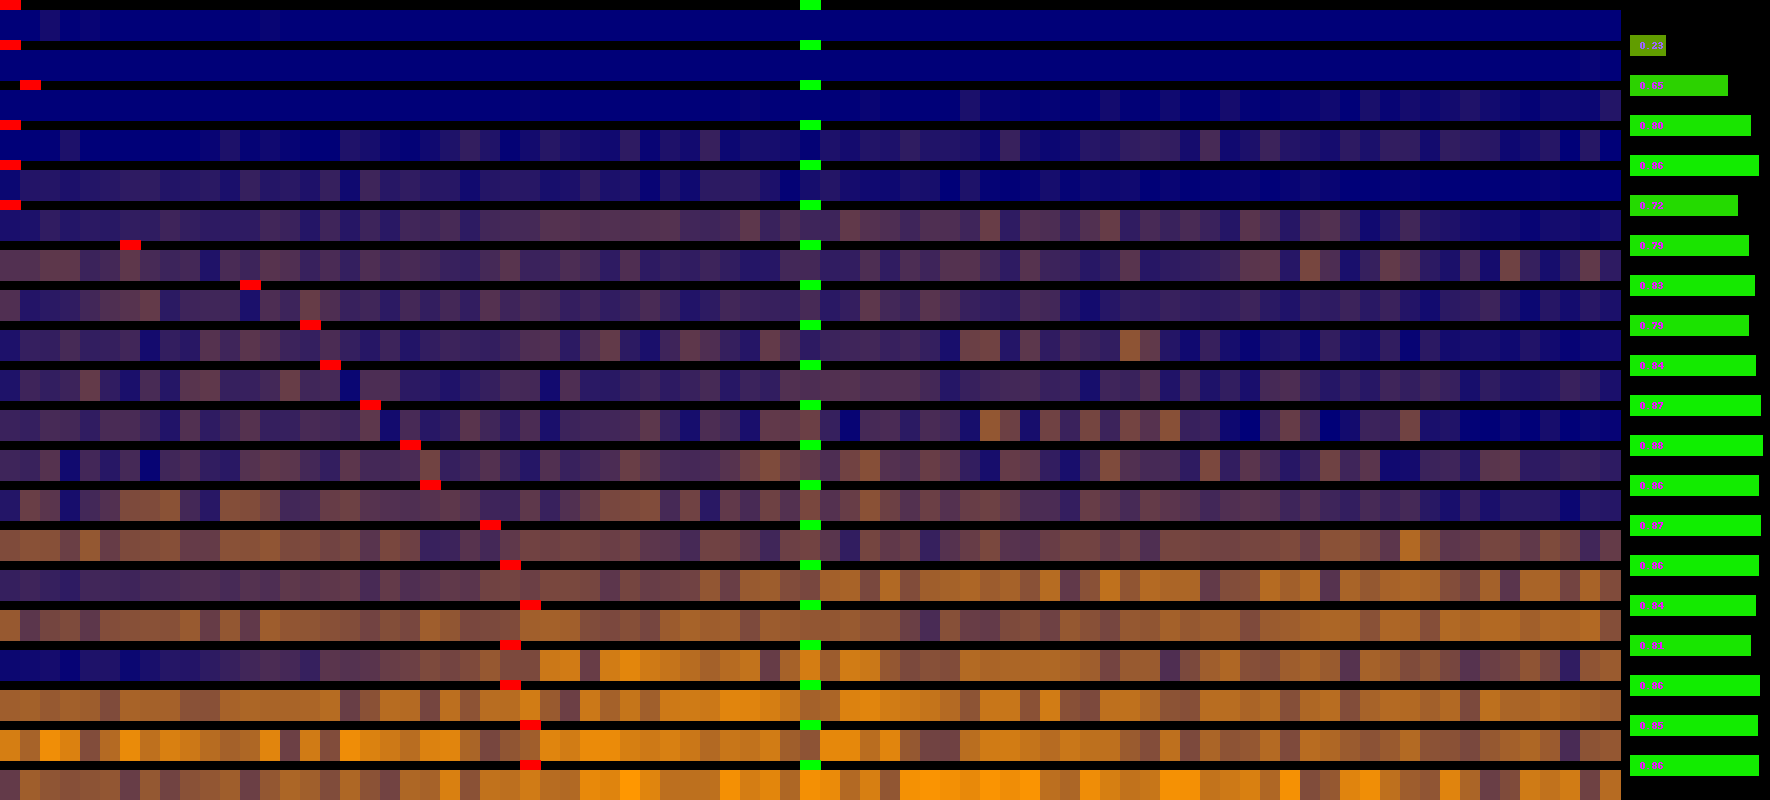
\includegraphics[width=10cm]{Images/gradientStudy}
    \caption{Un exemple de sortie de l'étude de gradient, environnement \emph{Pendulum}}
    \label{fig:gradientStudy}
\end{figure}

Pour avoir une idée de la distance parcourue entre chaque pas, on indique la position relative des modèles sur les droites : en rouge la position au pas précédent, en vert la position au pas actuel. \\

De plus, pour avoir une idée du changement d'angle entre chaque pas, on calcule le produit scalaire entre chaque direction. Il est affiché sur le côté de l'image. \\

% IMAGE GradientStudy from above
\begin{figure}[htp]
    \centering
    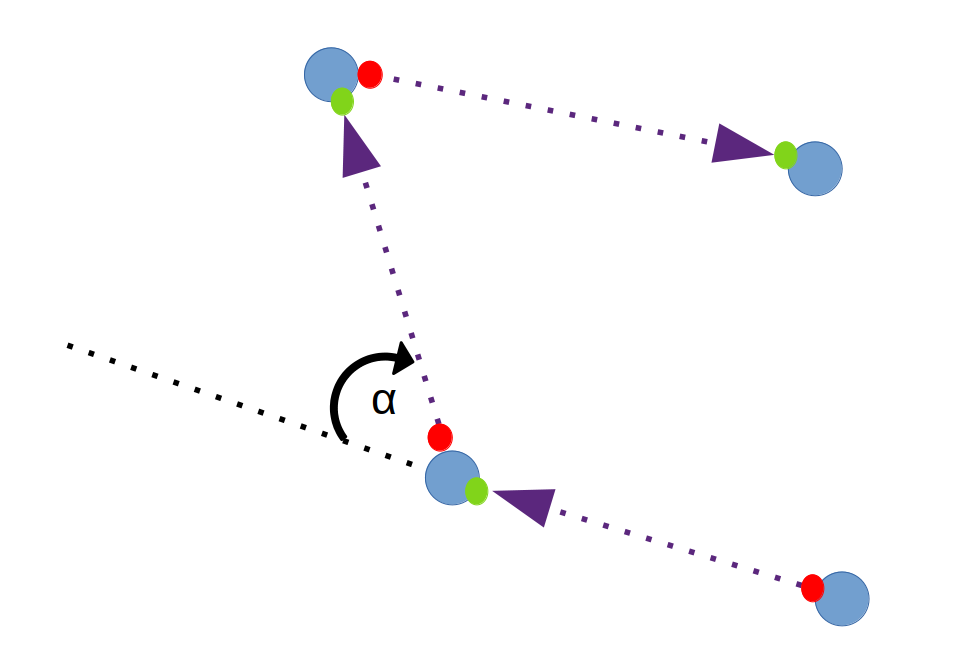
\includegraphics[width=10cm]{Images/gradientStudy_dessus}
    \caption{Descente de gradient en 2D, les lignes calculées correspondent aux flèches}
    \label{fig:gradientStudyAbove}
\end{figure}

Ainsi, cet outil permet de se représenter la trajectoire prise par un modèle lors de son apprentissage. \\

\newpage
\subsection{Vignette}

L’outil Vignette permet d’obtenir un aperçu des alentours d’un modèle. \\

% Méthode Muller ?
Il consiste à échantillonner l’espace d’apprentissage grâce aux droites introduites précédemment. \\

A partir du modèle initial, on obtient un aperçu d'une boule fermée en tirant des droites partant dans des directions aléatoires. \\

% IMAGE Vignette principle
\begin{figure}[htp]
    \centering
    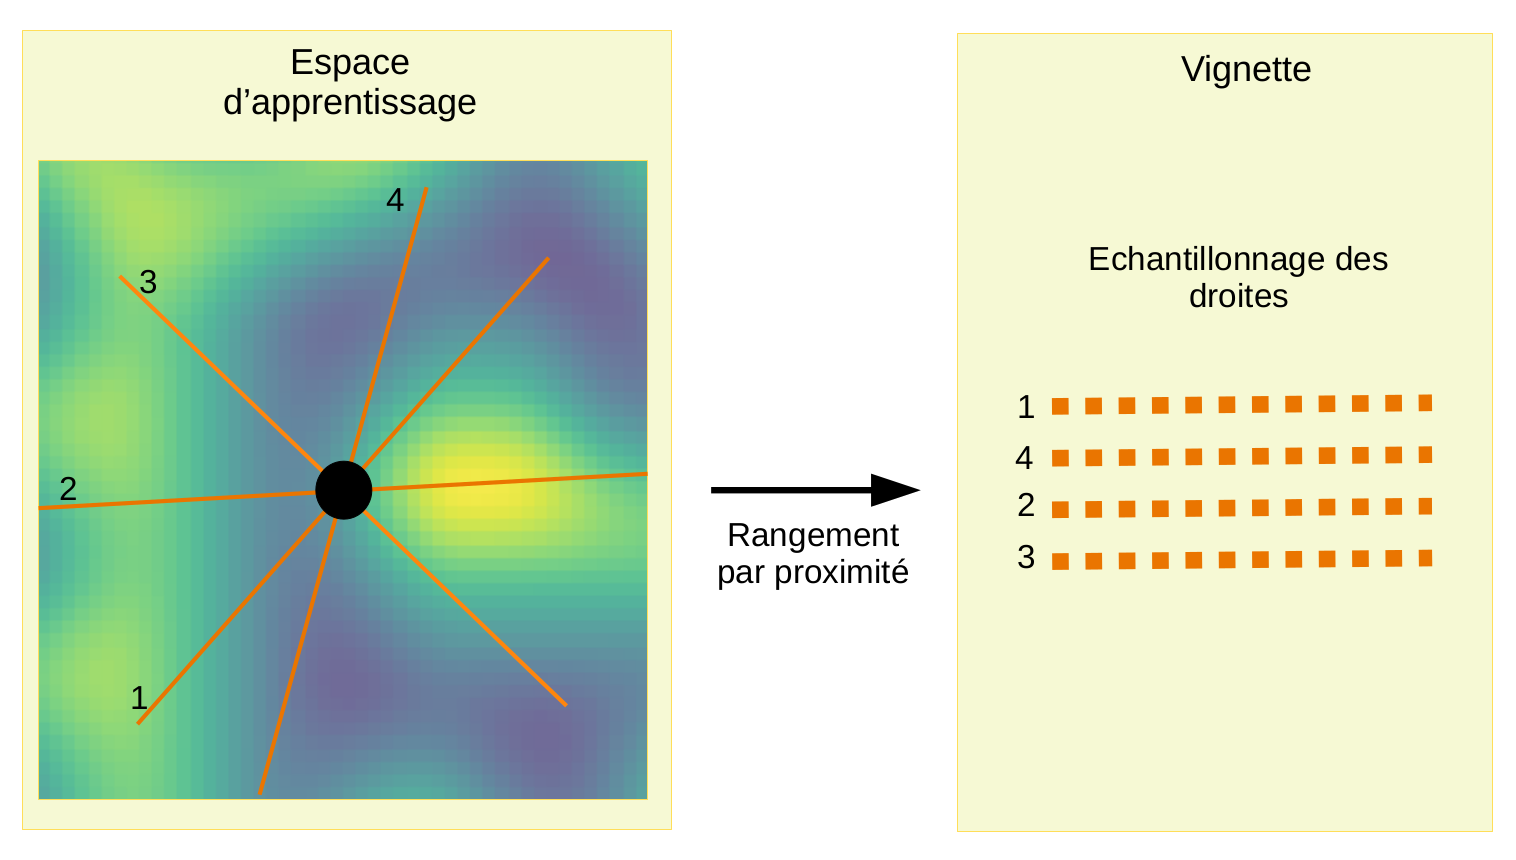
\includegraphics[width=12cm]{Images/VignetteDessin}
    \caption{Tirage des directions de Vignette}
    \label{fig:vignetteDessin}
\end{figure}

Les directions tirées aléatoirement sont alors triées par ordre de proximité, donnant un meilleur aperçu des structures. \\

% IMAGE Vignette real
\begin{figure}[htp]
    \centering
    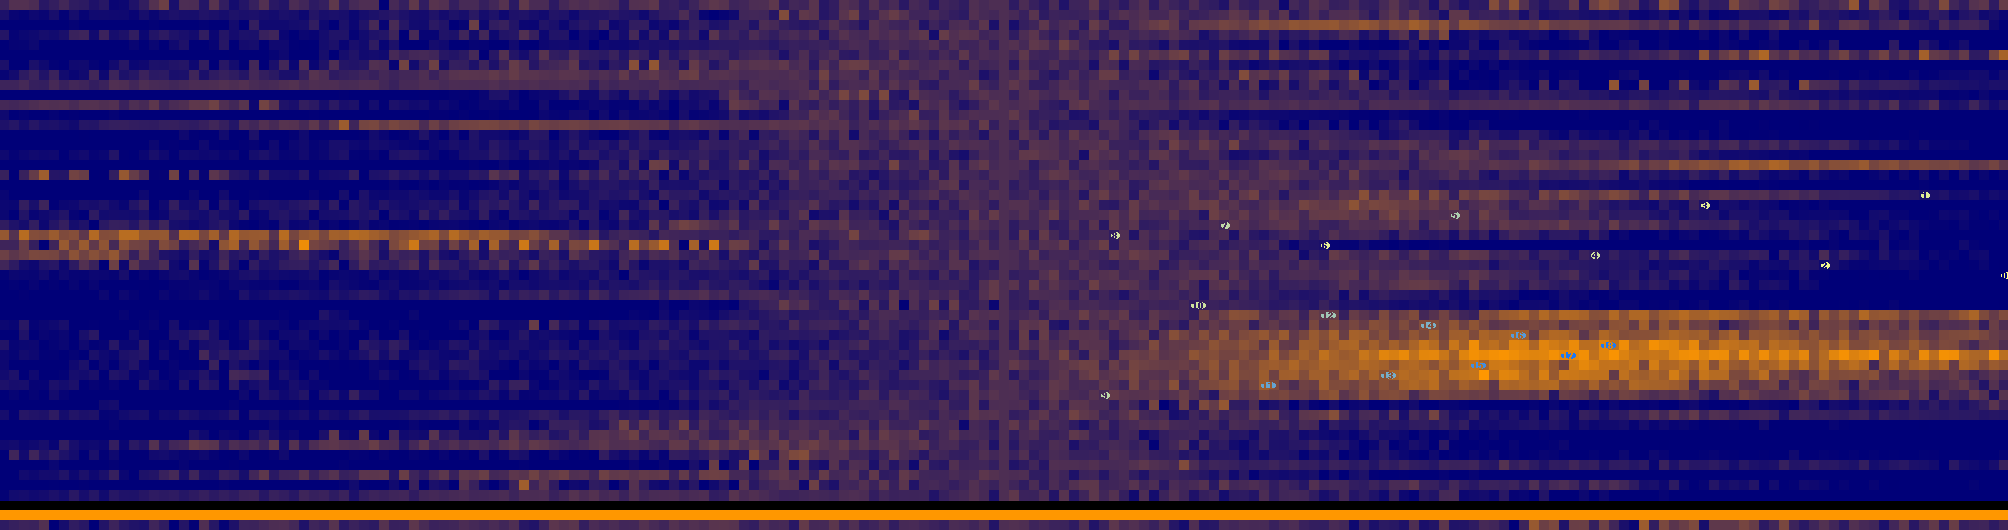
\includegraphics[width=12cm]{Images/Vignette_pendulum}
    \caption{Vignette 2D, 50 directions, environnement \emph{Pendulum}}
    \label{fig:vignetteDessin}
\end{figure}

On obtient alors une représentation en 2D de l’espace d’apprentissage, qui était alors en grande dimension (de la taille du réseau de neurones). \\

On observe bien la conservation des structures de l'espace d'apprentissage dans la Vignette, avec l'apparition d'ensembles de même récompense. \\

Notons que du fait du faible nombre de directions tirées par rapport à la dimension de l'espace, et de la discretisation des droites, cette représentation n’est que partielle. Il est possible que la Vignette passe à côté de structures ou de zones de rebroussement de gradient. \\

\newpage
\section{Nouvelles fonctionnalités}

Lors de notre projet, nous avons fait le choix d'offrir à l'utilisateur toutes les fonctionnalités nécessaires pour effectuer une analyse complète du paysage de valeurs d'un environnement et d'un algorithme. \\

Ainsi, nous proposons un ensemble de fonctionnalités permettant d'aller de l'entraînement d'un modèle jusqu'à l'affichage des résultats. \\

% IMAGE Architecture projet
\begin{figure}[htp]
    \centering
    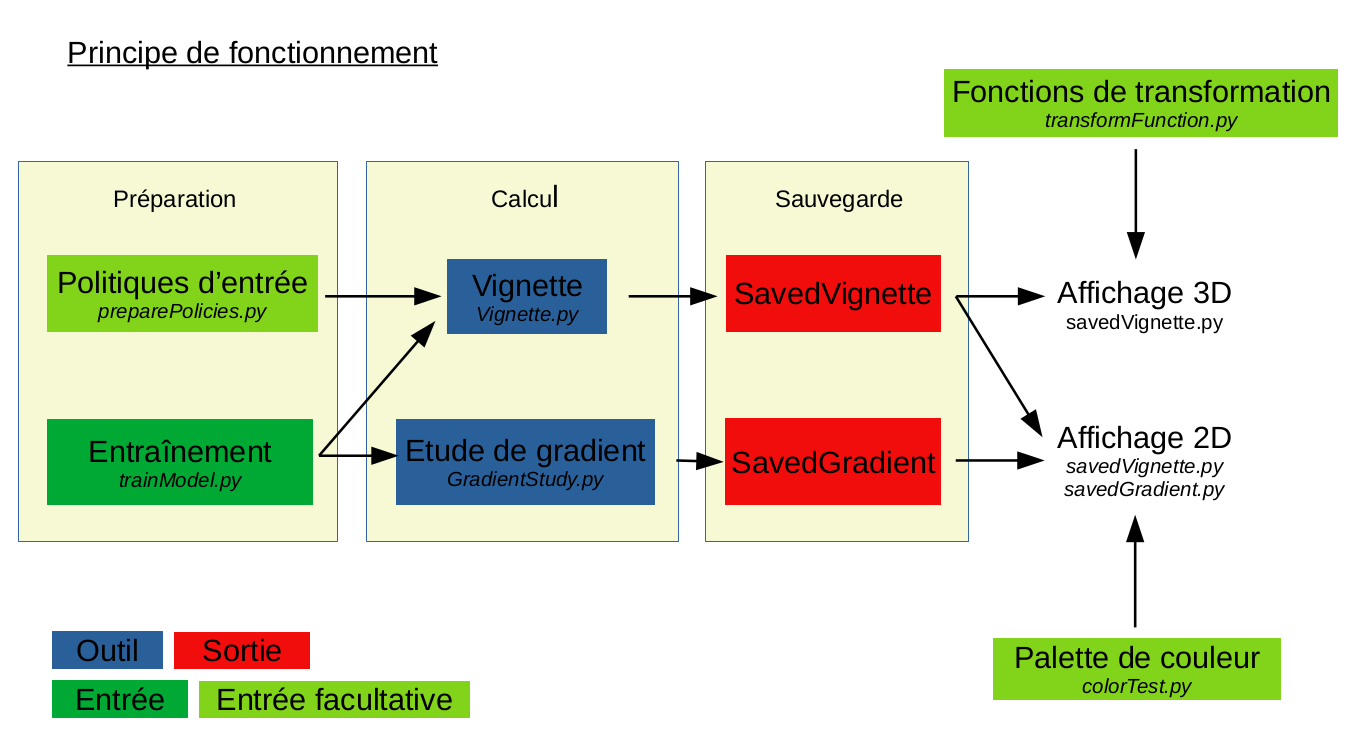
\includegraphics[width=18cm]{Images/Principe}
    \caption{Processus d'utilisation des outils}
    \label{fig:principe}
\end{figure}

L'utilisation des outils s'effectue en trois phases : 
\begin{itemize}
	\item préparation des entrée
	\item calcul de la Vignette ou de l'étude de gradient
	\item sauvegarde des paysages calculés
	\item utilisation des sauvegardes pour l'affichage
\end{itemize}

Dans cette partie, nous détaillerons chacune de ces phases.

\newpage
\subsection{Portage à \emph{stable-baselines-3}}

Lors de nos travaux, nous avons été contraints de réécrire le code des outils. \\

En effet, celui-ci était écrit pour fonctionner sur un environnement particulier (Mujoco Swimmer) sous l’algorithme TD3. \\

Nous avons procédé à un portage vers la librairie Stable-baselines-3, comportant un ensemble fiable d’implémentations d’algorithmes d’apprentissage par renforcement en PyTorch. \\

Le code de Stable-baselines-3 est accessible sur github et propose une documentation détaillée de ses implémentations. \\

Ainsi, pour chacun des outils il est possible pour l’utilisateur de changer facilement l’algorithme d’apprentissage, ses hyper-paramètres et l’environnement utilisé. \\

\subsection{Phase de préparation}

Avant toutes choses, pour fonctionner, les outils ont besoin de recevoir en entrée un modèle entraîné sous forme de réseau de neurones. \\

Grâce à leur implémentation sous \emph{stable-baselines-3 (SB3)}, les outils peuvent recevoir n'importe quel réseau de neurones au format PyTorch. \\

Nous proposons un exemple d'application de \emph{SB3} dans le fichier \emph{trainModel.py}. L'utilisateur peut alors entraîner un réseau de neurones sous l'environnement souhaité, en sauvegardant les étapes de l'apprentissage à une fréquence choisie. \\

De plus, l'étude portant sur une descente de gradient, il est nécessaire que l'utilisateur puisse fournir en entrée de Vignette une liste de politiques. Il peut alors observer la position relative de chacune des politiques de la liste avec la politique centrale de la Vignette. \\

% IMAGE politiques comparaison
\begin{figure}[htp]
    \centering
    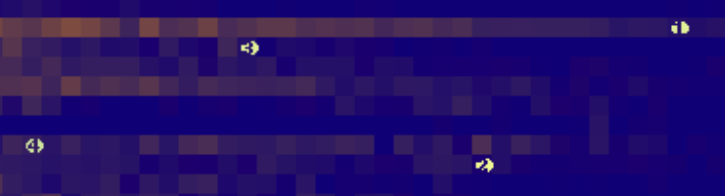
\includegraphics[width=10cm]{Images/politiques_entrees_vignette}
    \caption{Extrait d'une Vignette en affichant les politiques d'entrée}
    \label{fig:exempleEntree}
\end{figure}

\newpage

Nous détaillerons comment ces politiques d'entrée sont prises en compte lors du calcul de Vignette dans la partie suivante. \\

\subsection{Phase de calcul}

\emph{L'étude de gradient} prend en entrée un ensemble de politiques, correspondant à la progression de la descente de gradient pour le modèle entraîné. \\

Il calcule comme décrit précédemment, un suivi de la descente de gradient effectuée par le modèle. \\

% IMAGE gradientStudy Swimmer
\begin{figure}[htp]
    \centering
    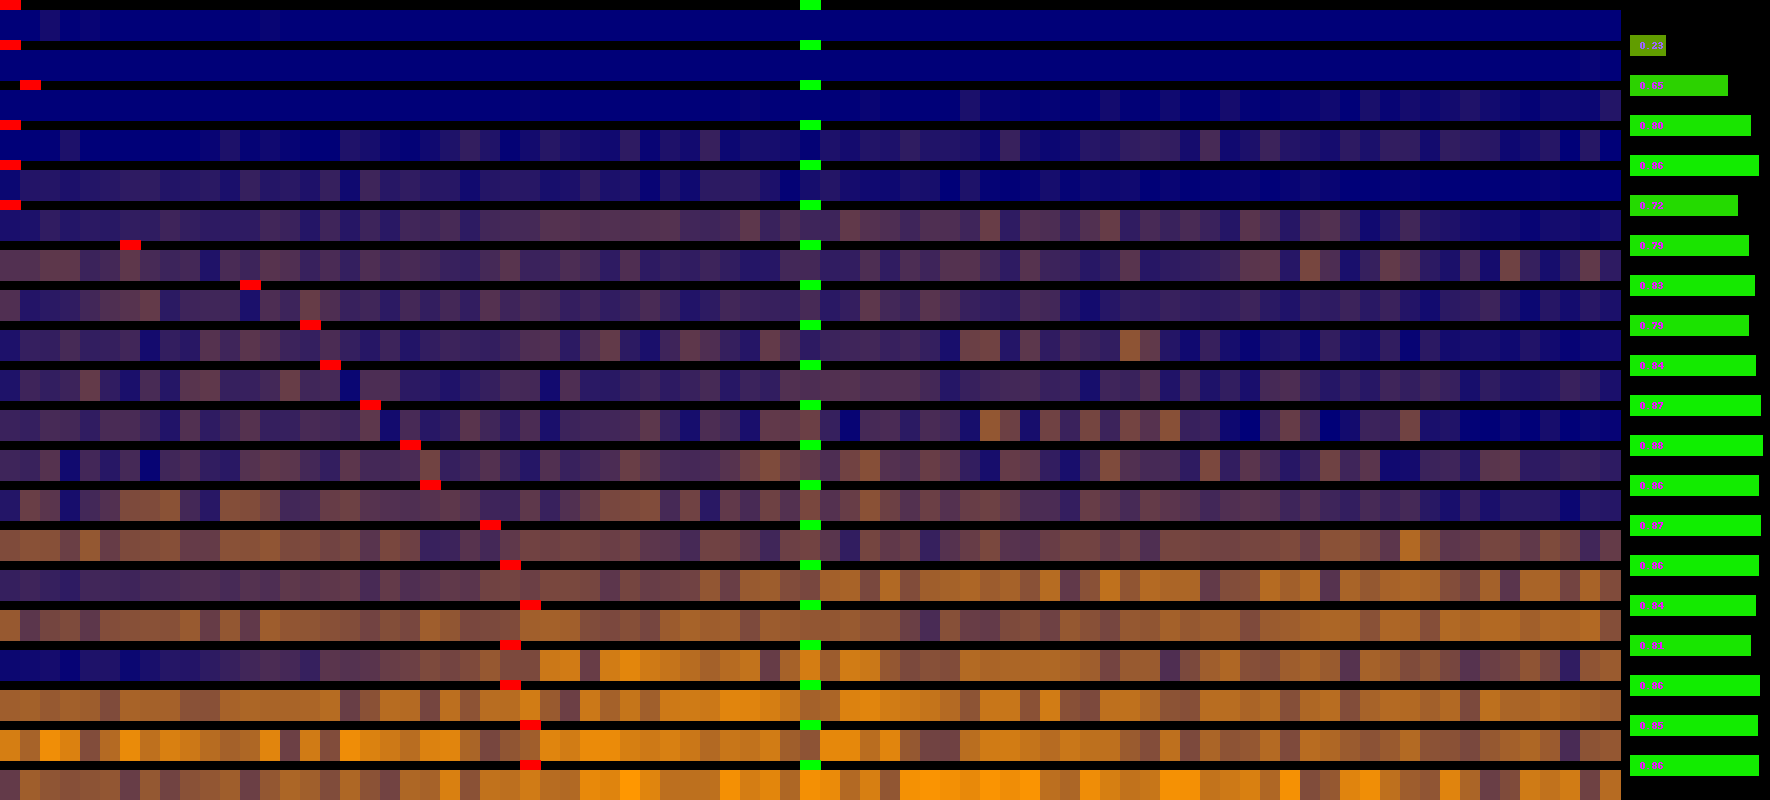
\includegraphics[width=10cm]{Images/gradientStudy}
    \caption{Etude de gradient sur Pendulum de 500 à 10000 pas, tous les 500 pas}
    \label{fig:gradientStudy}
\end{figure}

\newpage

Pour \emph{Vignette} la possibilité d'entrer une liste de politiques à situer sur la Vignette rajoute des étapes de calculs. La prise de celles-ci s'effectue en deux étapes. \\

Tout d'abord, rappelons que l'utilisateur donne en argument de Vignette une fréquence d'échantillonnage. Cette fréquence correspond à la résolution de chaque ligne. \\

Par conséquent, Vignette dispose d'une portée limitée. On ne peut observer qu'un aperçu de la boule fermée ayant pour centre le modèle central, et un rayon résultant de la résolution choisie. \\

Il est possible que des politiques d'entrée soient en dehors de cette boule. \\

Nous avons donc fait le choix d'imposer une baisse automatique de la fréquence d'échantillonnage de façon à atteindre toutes les politiques. \\

% IMAGE vignette portée
\begin{figure}[htp]
    \centering
    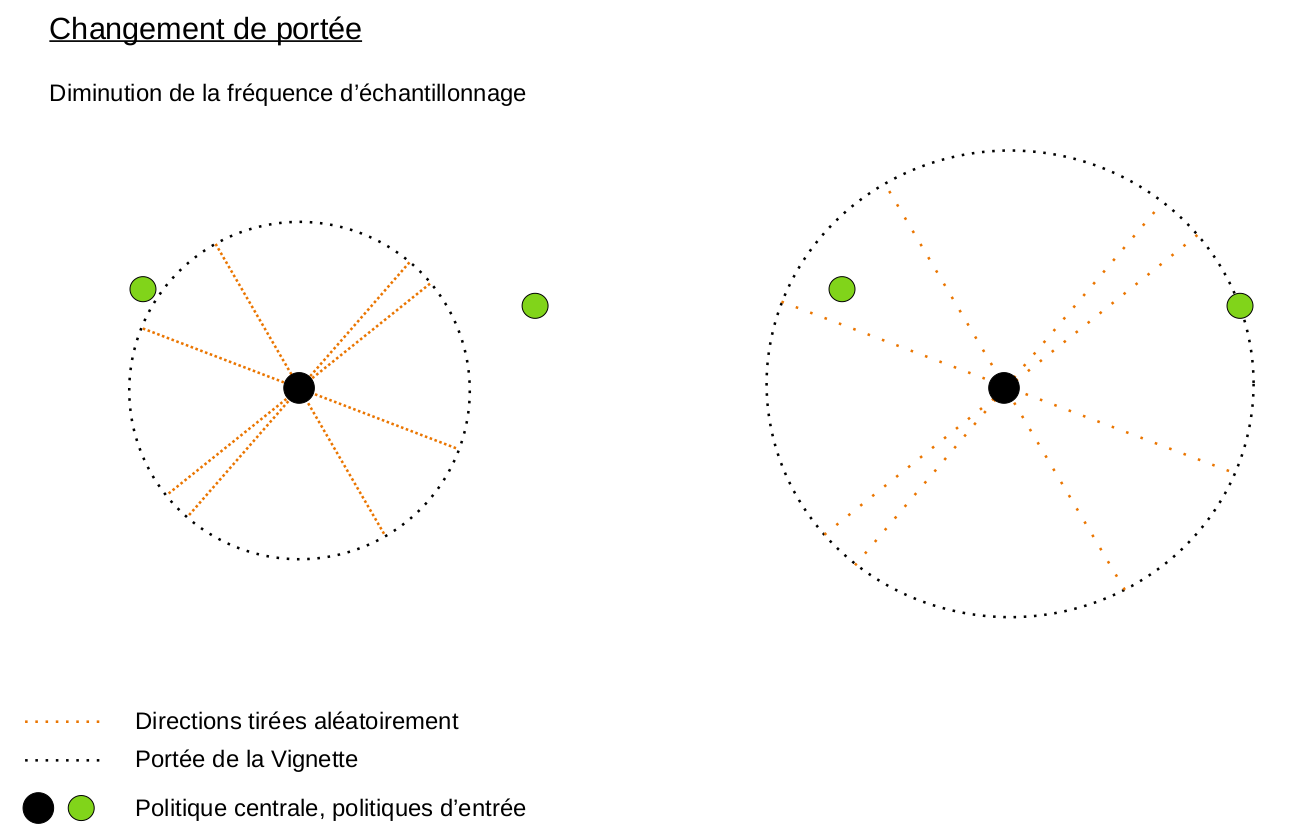
\includegraphics[width=15cm]{Images/vignette_portee}
    \caption{Première étape : ajustement de la portée}
    \label{fig:vignettePortee}
\end{figure}

Toutes les politiques sont alors présentes dans la boule fermée de la Vignette. \\

\newpage
La seconde étape consiste à insérer les directions passant par celles-ci dans le résultat final. \\

Le nombre de lignes tirées (la hauteur de la Vignette) étant un paramètre de l'utilisateur, il convient de remplacer certaines de ces lignes (donc directions) par celles correspondant aux politiques d'entrée. \\

Pour que l'introduction de ces politiques bouleverse le moins possible la Vignette d'origine, on insère les directions correspondentes à la place des directions qui en était les plus proches. \\

% IMAGE vignette directions
\begin{figure}[htp]
    \centering
    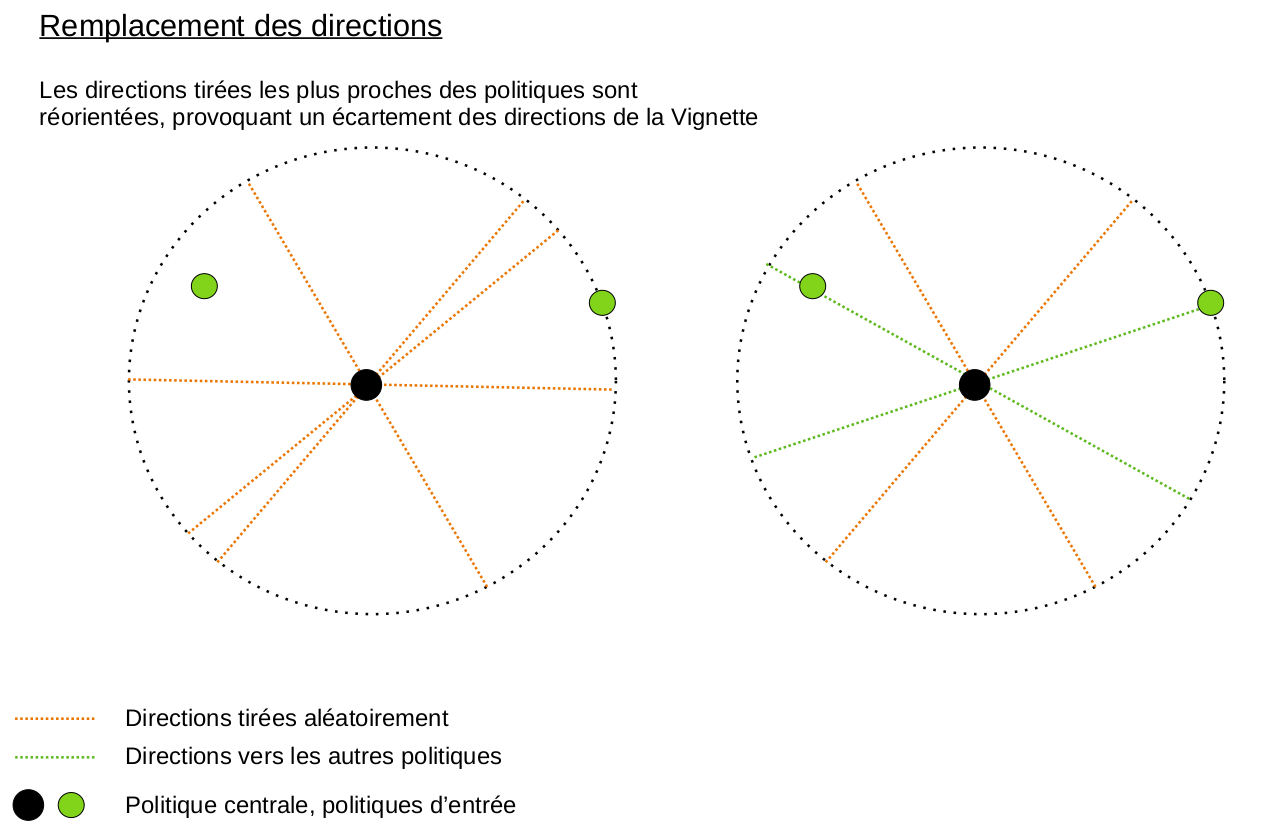
\includegraphics[width=15cm]{Images/vignette_portee2}
    \caption{Seconde étape : insertion des directions}
    \label{fig:vignettePortee}
\end{figure}

On constate dans l'exemple du dessin que cette étape a tendance à écarter les directions les unes des autres. Autrement dit, on étale l'espace balayé par la Vignette. \\

Cela a pour inconvénient de provoquer des discontinuités dans la détection de structures. Au contraire, l'utilisateur pourrait préférer concentrer les directions dans des faisceaux, permettant un meilleur niveau détail autour de directions particulières. \\

Une solution pourrait être de, au lieu de choisir la direction la plus proche, prendre la direction la plus isolée et la remplacer par la direction vers la politique. \\

C'est un problème flagrant dans notre représentation 2D simplifiée de l'espace d'apprentissage. Mais en réalité, le nombre de directions tirées est bien inférieur à la dimension de l'espace, ce qui réduit l'importance du problème. \\

\subsection{Phase de sauvegarde}

Une fois les calculs effectués, les données sont sauvegardées (serializées) dans un objet de type \emph{SavedVignette} ou \emph{SavedGradient}. \\

Chacun de ces objets garde en mémoire les directions ayant servies aux calculs, la valeur des récompenses pour chaque pixel. Permettant un traitement ultérieur des données si l'utilisateur le souhaite. \\

L'inconvénient de cette approche est qu'elle prend beaucoup de place en mémoire. \\

Nous utilisons une compression au format \emph{.xz} (algorithmes \emph{LZMA/LZMA2}). Bien que ce format soit relativement lent pour la compression, il est très rapide en décompression. \\

Cela le rend idéal pour notre application : la lenteure de compression est négligeable par rapport au temps de calcul des outils (quelques secondes contre quelques heures), mais la rapidité de décompression est parfaite car l'utilisateur sera ammené à fréquemment charger les résultats (pour faire des essais de modification des attributs par exemple). \\

La taille d'un fichier sauvegardé est de l'ordre de 100Mb. \\

\newpage
\subsection{Phase d'affichage}

Tout comme dans la version des années précédentes, nous offrons la possibilité d'afficher les résultats en tant qu'image 2D. \\

De plus, grâce à la fonctionnalité de sauvegarde nous avons pu implémenter une gestion des palettes de couleur. \\

Nous avons constaté que cette gestion des couleurs était utile. En effet elle permet aux personnes malvoyantes de régler le contraste des couleurs. De plus, certains écrans ont du mal à distinguer les faibles variations d'intensité de couleur entre les pixels. \\

% IMAGE différentes palettes
\begin{figure}[htp]
    \centering
    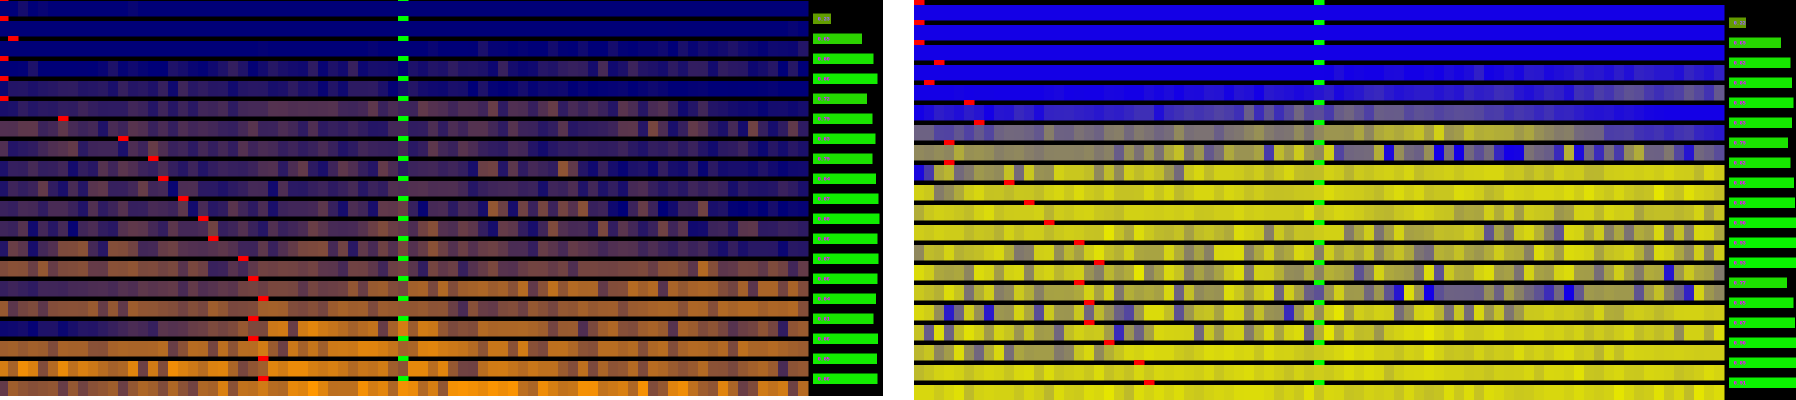
\includegraphics[width=10cm]{Images/palette}
    \caption{Différentes palettes de couleur}
    \label{fig:palette}
\end{figure}

La majeure partie de nos travaux a consisté à développer une visualisation en 3D de l'outil Vignette. Chaque pixel prend comme hauteur la récompense obtenue. \\

% IMAGE Vignette 3D
\begin{figure}[htp]
    \centering
    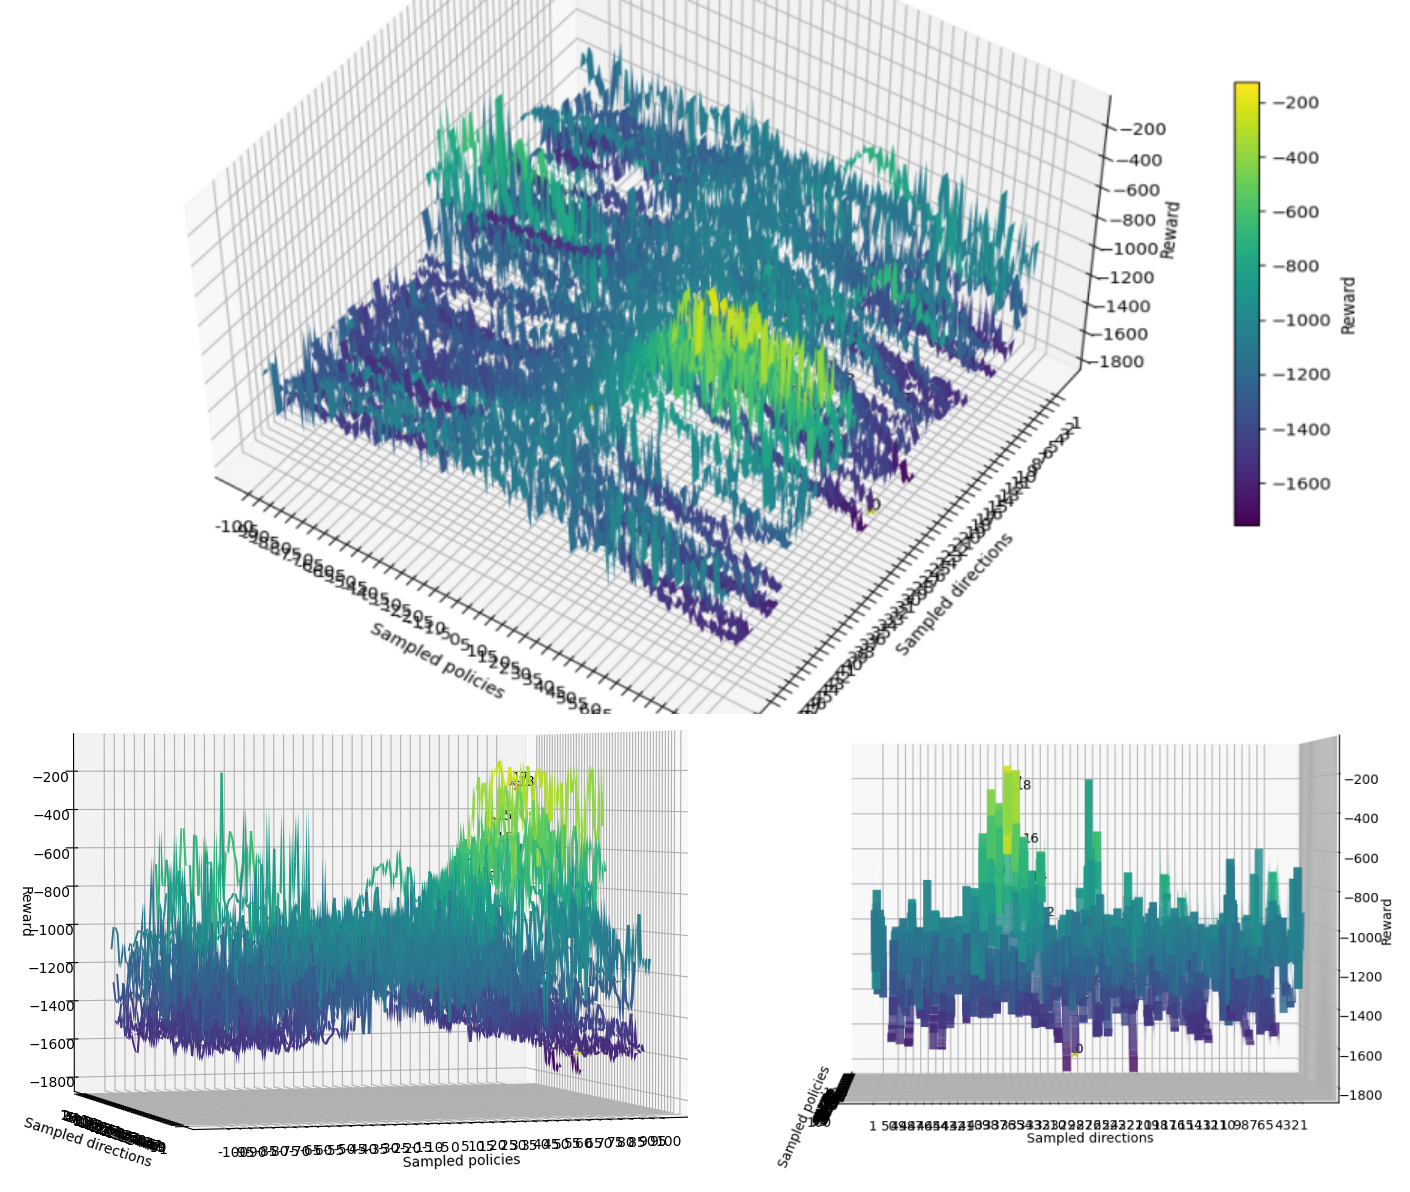
\includegraphics[width=8cm]{Images/vignette_3D}
    \caption{Vignette 3D, 50 directions, environnement \emph{Pendulum}}
    \label{fig:vignette3D}
\end{figure}
\newpage
Cette visualisation contient bien les mêmes informations que la version en 2D, cependant elle permet une approche plus intuitive de la structure de l'espace échantillonné. \\

On remarque qu'en vue de dessus on retrouve la Vignette en 2D. \\

% IMAGE vue de dessus
\begin{figure}[htp]
    \centering
    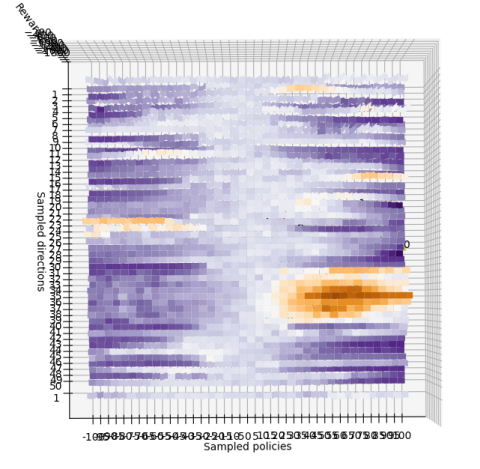
\includegraphics[width=10cm]{Images/vignette_dessus}
    \caption{Vue de dessus de Vignette 3D, on retrouve la Vignette 2D}
    \label{fig:vignetteDessus}
\end{figure}

Nous avons ajouté un curseur permettant de changer l'opacité des surfaces par soucis de visibilité. \\

On peut maitenant aperçevoir les politiques d'entrée de Vignette. \\

% IMAGE politique descente gradient + autre point de vue
\begin{figure}[htp]
    \centering
    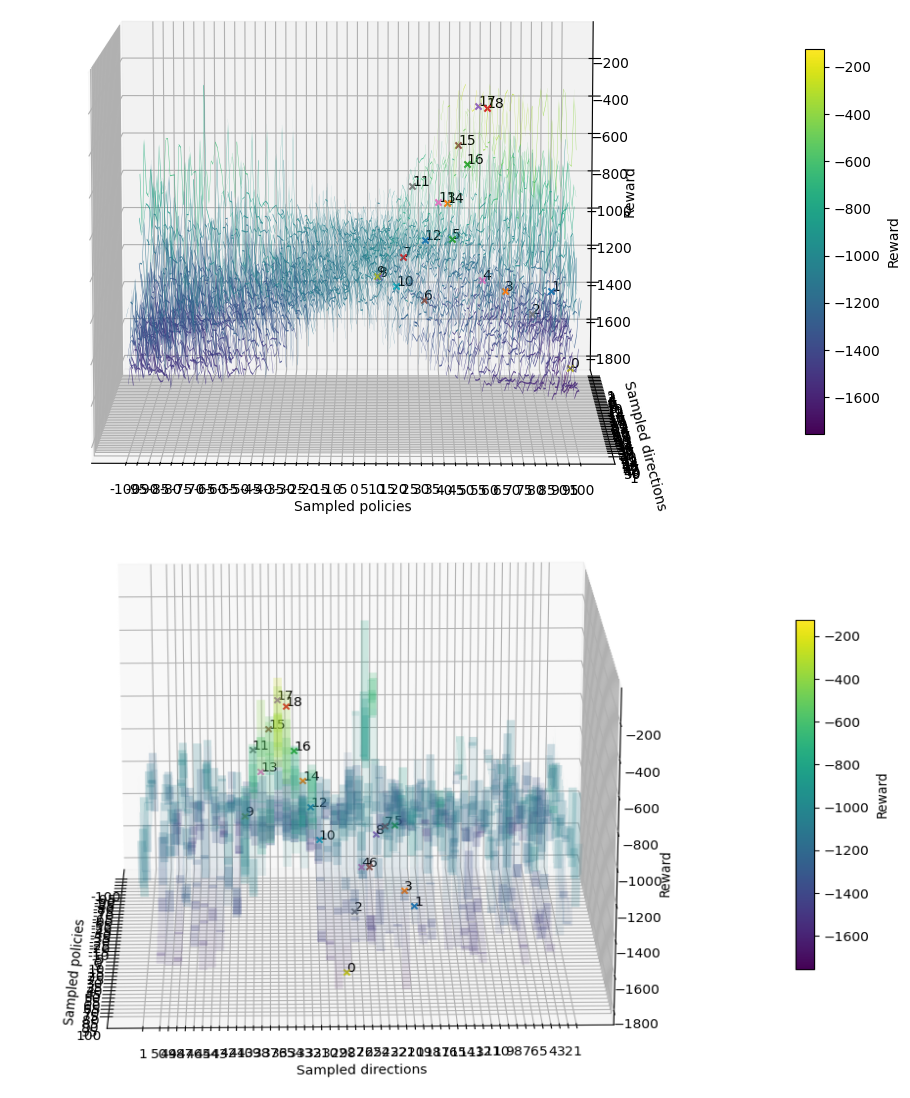
\includegraphics[width=15cm]{Images/vignette_cote}
    \caption{Vue de côté de la Vignette3D, on observe la descente de gradient}
    \label{fig:vignetteCote}
\end{figure}

\newpage
La Vignette ci-dessus correspond à une entraînement de Pendulum sur 10000 pas de temps enregistré tous les 500 pas. \\

La politique centrale est le pas de temps n°5000, est les politiques d'entrée correspondent aux 19 autres enregistrements du n°500 au n°10000. \\

Dans l'image vue de côté, on observe clairement le processus de montée de gradient : \emph{Pendulum} se déplace vers des zones de plus en plus hautes (amélioration de la récompense). \\

\subsection{Notes sur les fonctions de transformation : \emph{transformFunction}}

%% Peut être pas la place

\subsection{Accessibilité}

D’autres améliorations ont été apportées, notamment l’ajout de barres de progression pour l’utilisateur. Il a désormais une idée plus précise de la quantité de temps restante pour les calculs. \\

De plus, le code a été clarifié et largement commenté, il est maintenant facilement compréhensible par l’utilisateur. \\

\section{Exemples d'utilisation des outils}

Les outils sont à un stade de développement assez avancé pour être utilisés dans d'autres projets. \\

Nous avons d'ailleurs mis à disposition un mode d'emploi détaillant leur utilisation pas à pas. Celui-ci fait office de cahier des charges du projet. \\

\subsection{Projets utilisant Vignette}
Lors de nos travaux, nous avons bénéficié des retours d'autres groupes travaillant sur nos outils. \\

Par exemple, [... résumé Hector et Damien] \\

% IMAGE Hector et damien

\subsection{Régularisation de l'entropie}

\subsection{Stratégies de quadrillage de l'espace}
% Stratégies

\section*{Conclusion}
% Améliorations : interrompre et sauvegarde reprendre Vignette, Vignette calcul parallèle, nouvel outil faisceaux
\end{document}
